% !TEX program=xelatex

\documentclass{scrartcl}

\usepackage{polyglossia, xltxtra}
\setmainlanguage{german}
\usepackage{amsmath,mathtools, amsthm, amssymb,cases}
\usepackage{xcolor}
\usepackage{booktabs}
\usepackage{nicefrac}
\usepackage{multirow}
\usepackage{csquotes}
\usepackage{subcaption}
\usepackage[loadonly]{enumitem}
\newlist{arrowlist}{itemize}{1}
\setlist[arrowlist]{label=$\Rightarrow$}

\usepackage{scrlayer -scrpage}
\lohead{Mansur Daschaew \\ Janina Rastetter \\ Maren Raus}
\cohead{Prävalenzabhängige Kontaktdaten}
\rohead{14.02.2022}
\pagestyle{scrheadings}

\graphicspath{{img/}}

%\definecolor{theme}{rgb}{0.14,0.43,0.74}


%\newtheorem{defi}{Definition}[section]
%\newtheorem{satz}[defi]{Satz}
%\newtheorem{cor}[defi]{Korollar}
%\newtheorem{bem}[defi]{Bemerkung}
%\newtheorem{folg}[defi]{Folgerung}
%\newenvironment{beweis}
%	{\begin{proof}[Beweis]}
%	{\end{proof}}

\begin{document}

\begin{center}
\huge\textbf{Modellierung eines verallgemeinerten SEIR-Modells mit prävalenzabhängigen Kontaktraten}
\end{center}

\section{SEI\textcolor{blue}{D}R-Modell}

Das SEI\textcolor{blue}{D}R-Modell wird durch das folgende System gewöhnlicher Differentialgleichungen beschrieben:
\begin{align*}
\frac{dS}{dt} &= -\beta \frac{SI}{N} \\[10pt]
\frac{dE}{dt} &= \beta \frac{SI}{N} - \alpha E \\[10pt]
\frac{dI}{dt} &= \alpha E - \gamma I \textcolor{blue}{- \delta I} \\[10pt] 
\frac{dR}{dt} &= \gamma I \textcolor{blue}{+ \gamma D} \\[10pt] 
\textcolor{blue}{\frac{dD}{dt}} &\textcolor{blue}{= \delta I - \gamma D}
\end{align*}

\begin{tabular}{rl}
	Übergangsrate $\alpha$:& Kehrwert der mittlere Latenzzeit \\
	Transmissionsrate $\beta$:& Übertragungen pro S-I Kontakt pro Zeit \\
	Erholungsrate $\gamma$:& Kehrwert der mittleren infektiösen Zeit\\
	Testrate $\delta$: &  Testrate für positive Individuen $\times$ Rate der positiven Testergebnisse
\end{tabular}

%%%%%%%%%%%%%%%%%%%%%%%%%%%%%%%%%%%%%%%%%%%%%%%%%%%
%
% Simulation eines Lockdowns
%
%%%%%%%%%%%%%%%%%%%%%%%%%%%%%%%%%%%%%%%%%%%%%%%%%%%

\section{Simulation eines Lockdowns}
\textbf{Problemstellung:}
\begin{itemize}
\item Kontakte werden nicht kontinuierlich, sondern zu einem bestimmten Zeitpunkt eingeschränkt.
\item Der Zeitpunkt des Sprungs ist von der Inzidenz abhängig.
\item Bedingung an $\beta$: 
	$\beta(t) =  \begin{cases} 
					\phi \beta_0 \text{ falls } I(t) > \tau N \\
					\beta_0 \text{\quad sonst}
				\end{cases}$
	, wobei $\phi \in (0,1)$  und $\tau \in (0,1)$
\end{itemize}
 \
\textbf{Auswirkung auf den Verlauf der Epidemie:}
\begin{figure}[h]
\begin{subfigure}[b]{0.495\textwidth}  
		\centering
		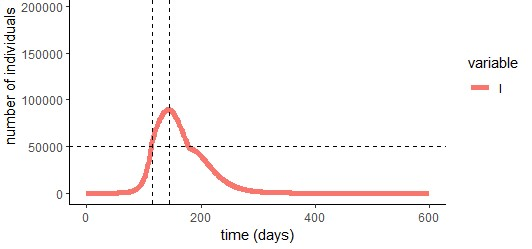
\includegraphics[width=\textwidth]{thres-I}  
		\caption{Anzahl der Infektionen bei Lockdown für $I(t) > 0.05N$}
	\end{subfigure}
        \begin{subfigure}[b]{0.455\textwidth}   
            \centering 
            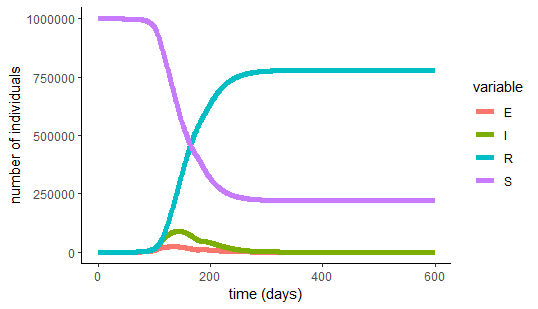
\includegraphics[width=\textwidth]{thres-epi}  
		\caption{Epidemieverlauf bei Lockdown für $I(t) > 0.05N$}           
        \end{subfigure}
 \end{figure}

\vspace{2cm}
\textbf{weitere Beobachtungen: }
\begin{itemize}
\item mehrstufiger Lockdown
\item Lockdownkriterium anhand der Fallzahlen anstatt der tatsächlichen Infektionen
\item adäquate Wahl der Schranke $\tau N$ notwendig
\item Zeitspannen zwischen Beginn des Lockdowns und Erreichen des Peaks
\end{itemize}


%%%%%%%%%%%%%%%%%%%%%%%%%%%%%%%%%%%%%%%%%%%%%%%%%%%
%
% Fallbeispiel Xi'an
%
%%%%%%%%%%%%%%%%%%%%%%%%%%%%%%%%%%%%%%%%%%%%%%%%%%%

\section{Fallbeispiel Xi'an}
	\begin{itemize}
		\item Beispiel für Chinas strikte Null-Covid-Strategie
		\item Einmonatiger Lockdown ab dem 23. Dezember 2021
		\item Annahme: nicht immunisierte Bevölkerung (plausibel aufgrund relativ wirkungsloser Vakzine)
	\end{itemize}

\subsection{Strategie 1: Keine Intervention}
	Verbleibende nicht infizierte Individuen: 0.7649229\% $\Rightarrow$ Durchseuchung
	\begin{figure}[h]
        	\centering
		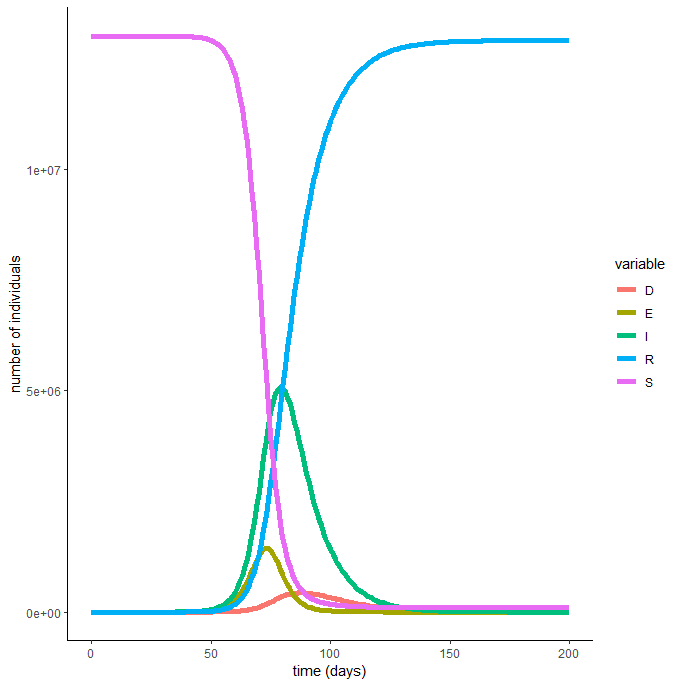
\includegraphics[scale=0.5]{delta=0,01,beta_unveraendert,alles.png}
		\caption{Verlauf mit $\delta = 0.01, \beta = \frac{5.5}{12}$}
	\end{figure}

\subsection{Strategie 2: Testen, testen, testen}
	\begin{table}[h]
		\caption{Verlauf mit verstärktem Testen}
		\centering
		\begin{tabular}{@{}ccc@{}}
			\toprule
			$\delta$ & Verbleibende S (in \%) & I und E kleiner 1, ab (in Tagen)\\ 
			\midrule
			 $\delta_{ur} \cdot 2^1$ & 1.252596 & 212 (+ 36) \\ 
			 $\delta_{ur} \cdot 2^2$ & 2.687945 & 196 (+ 36)\\  
			 $\delta_{ur} \cdot 2^3$ & 7.447852 & 186 (+ 36)\\ 
			 $\delta_{ur} \cdot 2^4$ & 23.80182 & 211 (+ 36)\\ 
			 $\delta_{ur} \cdot 2^5$ & 76.87228 & 589 (+ 36)\\ 
			 $\delta_{ur} \cdot 2^6$ & 99.93514 & 60 (+ 36)\\ 
			\bottomrule
		\end{tabular}
	\end{table}
	\begin{figure}[h]
        	\centering
		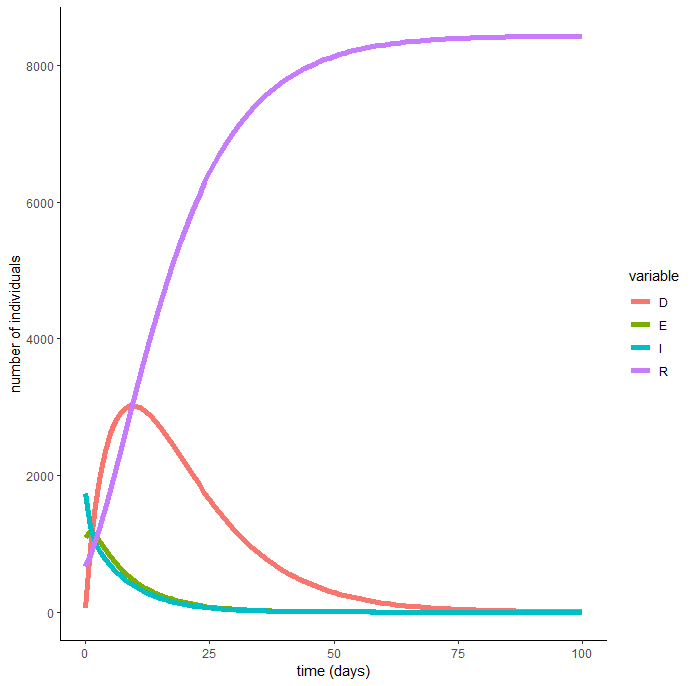
\includegraphics[scale=0.5]{delta=0,64,beta_unveraendert,ohne_s.png}
		\caption{Verlauf mit $\delta = 0.64, \beta = \frac{5.5}{12}$}
	\end{figure}	
	\begin{arrowlist}
		\item Erst ab einer Steigerung der Testeffizienz um Faktor $2^5$ ist eine Eindämmung der Epidemie möglich
		\item Bei einer Steigerung der Testeffizienz um Faktor $2^6$ müssten \enquote{nur} zwei Monate lang vermehrt getestet werden
	\end{arrowlist}

\subsection{Strategie 3: Kontaktreduktion}
	\begin{table}[h]
		\caption{Verlauf mit Kontaktreduktion}
		\centering
		\begin{tabular}{@{}ccc@{}}
			\toprule
			$\beta$ & Verbleibende S (in \%) & I und E kleiner 1, ab  (in Tagen)\\ 
			\midrule
			$\beta_{ur} * 2^{-1}$ & 11.3365 & 338 (+ 36) \\ 
			$\beta_{ur} * 2^{-2}$  & 65.28979 &  1184 (+ 36)\\  
			\nicefrac{1}{12} & 99.79345 & 898 (+ 36)\\ 
			\bottomrule
		\end{tabular}
	\end{table}
	\begin{figure}[h]
        	\centering
		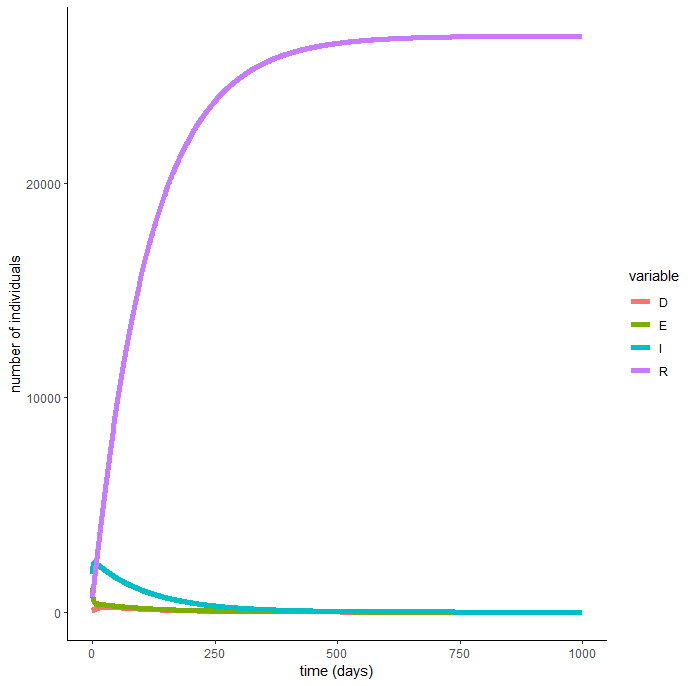
\includegraphics[scale=0.5]{delta=0,01,beta=1durch12,ohne_s.png}
		\caption{Verlauf mit $\delta = 0.0.1, \beta = \frac{1}{12}$}
	\end{figure}
	\begin{arrowlist}
		\item Kontaktreduktion verhindert Infektionen, zieht die Epidemie aber in die Länge
		\item Um eine Durchseuchung zu verhindern, müssten die Kontakte etwa 2.5 Jahre lang reduziert werden
	\end{arrowlist}

\subsection{Strategie 4: Kontaktreduktion und Massentests}
	\begin{table}[h]
		\caption{Verlauf mit verstärktem Testen und Kontaktreduktion}
		\centering
		\begin{tabular}{@{}ccc@{}}
			\toprule
			$\delta$ & Verbleibende S (in \%) & I und E kleiner 1, ab  (in Tagen)\\ 
			\midrule
			 $\delta_{ur} \cdot 2^1$ & 99.88242 & 456 (+ 36) \\ 
			 $\delta_{ur} \cdot 2^2$ & 99.92746 & 230 (+ 36)\\  
			 $\delta_{ur} \cdot 2^3$ & 99.95006 & 117 (+ 36) \\ 
			 $\delta_{ur} \cdot 2^4$ & 99.96137 & 60 (+ 36)\\ 
			 $\delta_{ur} \cdot 2^5$ & 99.96703 & 33 (+ 36)\\ 
			 $\delta_{ur} \cdot 2^6$ & 99.96986 & 20 (+ 36)\\ 
			\bottomrule
		\end{tabular}
	\end{table}
	\begin{figure}[h]
        	\centering
		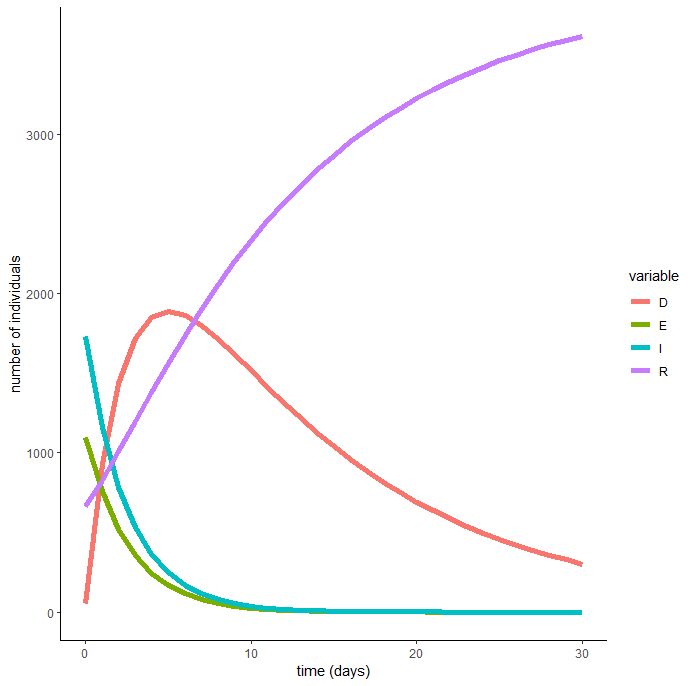
\includegraphics[scale=0.5]{delta=0,64,beta=1durch12,ohne_s.png}
		\caption{Verlauf mit $\delta = 0.64, \beta = \frac{1}{12}$}
	\end{figure}
	\begin{arrowlist}
		\item Bei extremer Kontaktreduktion wirkt sich die Testeffizienz kaum auf die Anzahl der Infektionen aus, dafür aber sehr stark auf die erforderliche Dauer der Beschränkungen
		\item Die Testeffizienz müsste mindestens um Faktor $2^4$ gesteigert werden, um die Dauer der Einschränkungen gering zu halten (ein bis zwei Monate)
	\end{arrowlist}

\subsection{Zusammenfassung}
	\begin{table}[h]
		\caption{Zusammenfassung}
		\centering
		\begin{tabular}{@{}ccccc@{}}
			\toprule
			Strategie & $\delta$ & $\beta$ & Dauer & Verbleibende S (in \%)\\ 
			\midrule
			-- & 0.01 & \nicefrac{5.5}{12} & 8.5 Monate & 0.7649229\\
			T &  0.64 & \nicefrac{5.5}{12} & 2 Monate & 99.93514\\ 
			K & 0.01 & \nicefrac{1}{12} & 2.5 Jahre & 99.79345\\
			K + T & 0.32 & \nicefrac{1}{12} & 1 Monat & 99.96703\\
			K + T & 0.64 & \nicefrac{1}{12} & 3 Wochen & 99.96986\\
			\bottomrule
		\end{tabular}
	\end{table}









\vspace*{\fill}
\textbf{Literatur:}  \\
P. Yan, G. Chowell: Quantitative Methods for Investigating Infectious Disease Outbreaks, 2019 \\
A. King: Ordinary differential equations in R, https://kinglab.eeb.lsa.umich.edu/480/nls/de.html, Zugriff: 03.02.2022

\end{document}